\documentclass{fose2016}           % for pLaTeX2e
%\documentclass[english]{fose2016} % for English papers
%\documentclass[ascii]{fose2016}   % for ASCII pTeX 

\usepackage[dvipdfmx]{graphicx}
%\usepackage{epsfig}

\title{依存関係の向きや開発者の属性が変更波及解析に与える影響の分析}
\etitle{Effects of Direction of Code Dependency and Attributes of Developers on Change Impact Analsys}% TODO dependency file, vector, develop time, impact analysis
\author{上田 裕己}{Ueda Yuki,島根大学総合理工学部}
\author{神谷 年洋}{Kamiya Toshihiro,島根大学総合理工学研究科}

\begin{document}

\maketitle

\begin{abstract}
変更波及解析はソースコードの依存関係を利用する分析手法のひとつである.
ソースファイルを対象とする変更波及解析の場合には,あるソースファイルが変更されると,そのソースファイルに依存している
ソースファイルの振る舞いも影響を受けるという仮説に基づき,テストや変更が必要になるソースファイルを予測する.
本研究では,依存関係の依存の向きに着目し,変更波及解析で仮定されている方向と逆向きの関係も含めて,
あるソースファイルの変更と,依存関係がある他のソースファイルの変更の時間間隔を,
オープンソースプロダクトのリポジトリを対象として調査した.
また,近年の分散開発においてはプロダクトの開発チーム外の
開発者が修正を行う(いわゆる「GitHubのプルリクエスト」)事例もあることに着目し,
変更を行った開発者によって依存関係と変更時間にどのような影響があるかも調べた.

\end{abstract}

%\begin{eabstract}

%\end{eabstract}

%はじめに
\section{はじめに} 
% 現在開発者の経験を図るために多くの研究で開発者がいままでに変更したファイルが利用されている.
ソフトウェアのモジュールと開発者の関係分析をソフトウェア開発プロセスに役立てる手法が研究されている\cite{Bird,Thongtanunam}.
Bird\cite{Bird}らは専門レベルという開発者があるファイルに対してどれだけ詳しいかという度合いによってソフトウェアの故障率に影響を与えるという研究を行った.
これにより,ソフトウェアプロジェクトの管理者は問題に対して最適な開発者を割り当てることができる.
しかし,変更が行われたファイルと依存関係にあるファイルに対して十分な検査が行えず,不具合を見逃す恐れがある.

変更波及解析はファイルの変更に対して,そのファイルに依存するファイルにも変更が必要になるのかを解析するモデルである.
既存研究では,依存関係の逆向きに変更の必要が起きる事例について議論したもの\cite{Beszedes}は少ない.
本研究では変更波及解析で仮定されている方向とは逆の変更されたファイルに依存されているファイルや間接的に依存関係のあるファイルに対しても調査することで,
従来議論されてこなかった依存関係を遡る向きの影響を調べる.

そのために,本論文では変更されたファイルに対して依存関係のあるファイルが変更されるまでの時間の間隔(以降,変更時間間隔,単位は日)への影響について調査を行った.
ある変更が行われてから,早い変更時間間隔で変更が行われるファイルには, 不具合が発生やリファクタリングが起きていると考えられる.
変更時間間隔を調査することにより,どのような依存関係のあるファイルに開発者が注目すればいいのかが,わかることが期待される.

調査の手法としては,対象とするソフトウェアプロジェクトにおいて,変更が行われたファイルに対して,プロジェクト内のすべてのファイルがどのような依存関係を持っているのか6つに分類を分けそれぞれの変更時間間隔への影響を調査する.
また,プロジェクトに権限を持っている人物による変更であることによる変更時間間隔への影響を調査するために,同じ人物が変更した場合,マージとなった変更の場合でも同様の調査を行った.

本論文では\ref{関連研究}章で関連研究について述べ,\ref{ツール・サービス}章では分散バージョン管理システム・サービスについて,\ref{アプローチ}章で問題へのアプローチ,\ref{調査対象のデータセット}章では調査対象のデータセットについて,\ref{実験}章で実験の内容と結果,\ref{考察}章で実験結果についての考察,\ref{妥当性の検証}章では実験の妥当性についての検証,最後に\ref{まとめ}章でまとめを行う.


%関連研究
\section{関連研究}\label{関連研究}
開発者はソフトウェアに対して多くの変更を行う.
その過程で,変更した部分だけでなく,変更されていない部分への振る舞いも変更してしまう可能性がある.
変更波及解析ではソフトウェアのモジュール間の依存関係を調べることで,変更の影響を受ける部分の識別が行う.
変更波及解析にはさまざまな手法が提案されているが\cite{Ryder,Kondo},本研究では変更による影響を受けたファイルを特定するため,ファイルと粒度の近いクラス単位での解析\cite{Ryder}を行う.
ソフトウェアの依存関係を評価する方法として,システムのモジュール間での依存関係をマトリクス表示するDSM(Dependency Structure Matrix)がある\cite{Nord}.
本論文ではこの評価方法と類似した方法により依存関係を求める.

% 利用したツール
%「分散バージョン管理システムにおけるバージョンの概念」や「プルリクエスト」を説明するものにしましょう.図1や図2の説明に繋がるように.
\section{分散バージョン管理システム・サービス}\label{ツール・サービス}
% git
\subsection{バージョン管理システム, git}
バージョン管理システムとはファイルの変更の履歴を保存するためのシステムである.
現在多くのソフトウェアではバージョン管理システムが利用されている.
今回調査を行ったvert.vプロジェクトも同様にバージョン管理システムの一つであるgitで管理されている.
gitなどの分散型のバージョン管理システムでは,多くの開発者が一つのソフトウェアを変更していても,変更の重複を防ぐことができる.
変更を記録することをコミットを呼び,コミットを利用することで前回のコミットから現在までに変更されたファイルを調べることができる.

gitで利用されているものにブランチがある.
ブランチは履歴の流れを分岐して記録していくためのものであり,同じプロジェクトの中で複数の変更を同時に進めていくことを目的としている.
有益な変更が行われたブランチの変更は主となるブランチであるmasterに統合される.これをマージという.
マージもコミットの一つであり,マージされることによりマージされたブランチにあったコミットはmasterのコミットとしても存在する.

% GitHub
\subsection{GitHub}
さまざまなオープンソースソフトウェアをにプロジェクトの構成員(開発者)の管理やgitによる バージョン管理システム,wikiなどの機能をホストしているサービスである.
これを利用してプロジェクトや開発者の状況を確認したり,ほかの開発者と議論をすることができる.

GitHubを用いたオープンソース開発プロジェクトの特徴として,プロジェクト外の開発者もGitHubにあるソースコードを別のブランチとして変更し,その変更を投稿することができる.
この投稿はプルリクエストと呼ばれている.
GitHub内でプルリクエストが投稿された時,コードレビューという,プロジェクト内の開発者(すなわち変更を行った開発者)とは別の開発者によるコードの査読が行われる.
このコードレビューでプロジェクト内の開発者が有用と判断した変更はmasterにマージされる.


% アプローチ
\section{アプローチ}\label{アプローチ}
変更波及解析では,2つのファイルf, gの間に,fがgに依存するという関係があるとき, gの変更されると,fはそれ自身は変更されなくても,gの変更の影響を振る舞いが変化してしまう可能性があるため, fに対するテストを再度行ったり,あるいは,fを変更する必要性があると判断する.本研究の目的は,GitHubのような,プロジェクト外の開発者も (プルリクエストという形で)ファイルを変更するようなプロジェクトの形態が,変更波及解析が同様に利用できるかを調べることである. そのために,プロジェクト内の開発者がファイルを変更した場合と, プロジェクト外の開発者がファイルを変更した(プロジェクト外の開発者が行った修正をプロジェクト内の開発者が取り入れた)場合とで,ファイルの修正のタイミングに影響がないかを調査する. より具体的には,
変更時間間隔に影響を受ける依存関係,開発者,gitの利用状況についての傾向を調査するために,以下の項目について調査を行う.
\begin{itemize}
\item RQ1:変更されたファイルに依存関係のあるファイルが変更されるまでの時間は依存関係のないファイルより短くなる.
\item RQ2:依存関係があるファイル(fがgに依存)の変更において,gが変更されたあとfが変更時間間隔は,fとgの開発者が同じ場合には,異なる場合よりも,短くなる.
\item RQ3:依存関係があるファイル(fがgに依存)の変更において,gが変更されたあとfが変更時間間隔は,fのコミットが複数のブランチのマージとなったコミットである場合には,そうではないコミットの場合よりも長くなる
\end{itemize}
% RQ1
\subsection{RQ1:変更されたファイルに依存関係のあるファイルが変更されるまでの時間は依存関係のないファイルより短くなる}
依存関係に種類を定義することによってどの種類がファイルの変更時間間隔に影響を与えるのか調査を行った.

ここでは,以下の仮説について調査を行う.
\begin{enumerate}
\item RQ1-1ファイルfがファイルgに依存するとき,gが変更されたあとfが変更されるまでの時間は,依存関係がないファイルと比較して短い
\item RQ1-2 ファイルfがファイルgに依存するとき,fが変更されたあとgが変更されるまでの時間は,依存関係がないファイルと同じである
\end{enumerate}

また,本研究ではソースコードのうち以下のような記述を依存関係として扱う.
変更が行われたファイルに対して以下の例のような記述が存在した場合,クラスAを定義しているファイルに依存しているとする.

\begin{itemize}
\item 参照による代入や呼び出し,定義(例:ClassA a = new ClassA())
\item 継承 (例: ClassB extends ClassA)
\end{itemize}

依存関係があるファイルにも依存関係の方向や間接的な依存関係をもつものを考慮するためにプロジェクト内のすべてのファイルに対し,与えられた変更を起点として表\ref{tab:依存関係の分類}に示したような分類を付与する.
本論文ではこの分類を依存関係の分類と呼ぶことにする.図\ref{fig:dependency}に依存関係の分類についての概要を示した.

\begin{table}
\begin{center}
\caption{依存関係の分類}
\begin{tabular}{|l|l|} \hline
分類名 & 概要 \\ \hline
root & 変更されたファイル \\ \hline
dependee & rootが依存するファイル \\ \hline
depender & rootが依存されるファイル \\ \hline
dependee2 & dependeeが依存するファイル \\ \hline
depender2 & dependerが依存されるファイル \\ \hline
other & 上記に当てはまらないファイル \\ \hline
\end{tabular}
\label{tab:依存関係の分類}
\end{center}
\end{table}

\begin{figure}[t]
\centering
\includegraphics[width=0.9\columnwidth]{dependency.pdf}
\caption{依存関係の分類図}
\label{fig:dependency} 
\end{figure}

% RQ2
\subsection{RQ2:依存関係があるファイル(fがgに依存)の変更において,gが変更されたあとfが変更時間間隔は,fとgの開発者が同じ場合には,異なる場合よりも,短くなる}
同一人物が変更を行った場合とそうでない場合でRQ1と同じく変更時間間隔への影響を調査した.
これを調べることにより,依存関係による影響を解決している人物はどのような依存関係に集中しているのか,
また,同じ開発者であることによって,どのような依存関係のあるファイルが影響を受けるかをRQ1と同様に調査する.

% RQ3
\subsection{RQ3:依存関係があるファイル(fがgに依存)の変更において,gが変更されたあとfが変更時間間隔は,fのコミットが複数のブランチのマージとなったコミットである場合には,そうではないコミットの場合よりも長くなる}
マージとなるコミットの場合はプルリクエストが投稿された後,コードレビューがされているコミットである可能性が高い.
これに対して,マージとなるコミット以外のコミットの場合, コードレビューを経ていない可能性が高い.
前者と後者の変更時間間隔を比較すると, 後者はコードレビューを経ていないため品質が低く,
よって,マージとなるコミットはそうでないコミットよりも変更時間間隔が長くなると考えた.

ここではマージされたコミット変更ではそうでない変更の変更時間間隔を,RQ1と同様に依存関係の分類別に,比較してどのような影響があるのか調査をする.

                                                                                                                                                                                                                                                                                                                                                                                                                                                                                                                                                                                                                                                                                                                                                                                                                                                                                                                                                                                                                                                                                                                                                                                                                                                                                                                                                                                 % 調査方法
\section{調査対象のデータセット}\label{調査対象のデータセット}
GitHub上のeclipseに関するプロジェクトの中で最もstar数が多かったvert.vプロジェクトを調査の対象とした.
vert.vプロジェクトは2013年から2016年まで変更され続け,合計2000以上のコミットが行われている.
eclipseプロジェクトには多くのオープンソースソフトウェアがあり,今後ほかのプロジェクトと比較するのに適していると考えたことも選定した理由のひとつである.

% コミットの分類
\subsection{コミットの分類}
本研究ではコミットの分類を以下の4つに分けた.

\begin{enumerate}
\item masterのコミット \label{enum:basedcommit}
\item masterのマージとなるコミット \label{enum:mergecommit}
\item マージされたブランチでmasterに\ref{enum:basedcommit}として取り込まれたコミット \label{enum:mergedbranch}
\item マージされていないブランチで行われたコミット
\end{enumerate}

図\ref{fig:gitimage} にコミットの分類を図示する.

\begin{figure}[t]
\centering
\includegraphics[width=0.8\columnwidth]{git_image.pdf}
\caption{gitによるコミットの分類分け}
\label{fig:gitimage} 
\end{figure}

本研究で分析するコミットは\ref{enum:basedcommit}と\ref{enum:mergecommit}のコミットである.
\ref{enum:mergedbranch}のコミットはマージされ\ref{enum:basedcommit}としてmasterに存在するため,\ref{enum:basedcommit}のコミットのみを分析する.

% データセット・取得データ
\subsection{取得データファイルの属性}
個々のソースファイルから表\ref{tab:初期データセット}に示す属性を取得した.

\begin{table}[htb]
\begin{center}
\caption{出力するデータセット}
\begin{tabular}{|l|l|} \hline
属性名 & 概要 \\ \hline
commit\_no & 最新のコミットの間に存在するコミット数 \\ \hline
file\_path & ファイルの絶対パス \\ \hline
date & 変更が行われた日付 \\ \hline
author & 変更を行った開発者の名前 \\ \hline
is\_merge & マージとなるコミットであるかどうか \\ \hline
\end{tabular}
\label{tab:初期データセット}
\end{center}
\end{table}

commit\_noとは最新のコミット該当するコミットの間にあるコミットの数を示している.データ型は数値型である.
file\_pathとは出力するファイルのファイルシステム上でのファイルパスである.
同一のcommitNoに対してその時点でのプロジェクトでのすべてのjavaファイルを出力している.
一つのファイルが表\ref{tab:依存関係の分類}で示した依存関係の分類に複数該当する場合があるため,主キーとはならない.
%このファイルパスは一意ではなく,同じfilepassとcommitNoでもkindが別のものがある.データ型は文字列型である.
%kidを使わない説明
dateとは変更が行われた日付を出力している.データ型は日付型である.
authorとは変更を行った開発者の名前を出力している.データ型は文字列型である.
%kindとは表\ref{tab:依存関係の分類}で示した依存関係の分類を出力している.データ型は文字列型である.
is\_mergeとはコミットがマージとなるコミットかどうかを分類しているものであり,論理型の値を得る.
図\ref{fig:gitimage}で示されているとおり,マージとなるコミットとマージではないコミットを識別している.

これらの情報をもとに,各ファイルfについて,fをrootとしたときの
f以外のファイルについて,fからの相対的な変更時間間隔を求める.
データ型は数値型,単位は日である.
%実験
\section{実験}\label{実験}

%実験・手順
\subsection{実装}
対象となるプロジェクトのgitレポジトリからデータを取得し,表\ref{tab:初期データセット}のデータを取得する処理の内容を以下に記す.
\begin{enumerate}
\item ファイルの絶対パスをキーとし,ファイルの属性を値とするテーブル(file\_path → 属性)を用意する.
\item 最新リビジョンを対象とする.
\item そのリビジョンのコミット番号を調べる(commit\_no).
\item そのリビジョンがマージされたブランチかを調べる(is\_merge).
\item そのリビジョンに含まれるファイルの集合をFとする.
\item Fに含まれる各ファイルについて,ファイルの絶対パス(file\_path),変更が行われた日付(date),変更を行った開発者の名前(author)を調べる.
\item Fに含まれるファイルのすべての組み合わせ(f, g)について,
\begin{enumerate}
\item fをrootとしたときのgの依存関係の種類を調べ\label{enum:依存関係の種類を調べる}
\item もしgがそのリビジョンで変更されていなくて,かつ,もしgがテーブルに含まれていれば,fとテーブルに記録されているgと同じパスのファイル(gの次のバージョンのファイル)との相対的な変更時間間隔を求める.
\item  もしgがそのリビジョンで変更されていて,fより後の日付で変更されていれば, fとgの変更の日付から相対的な変更時間間隔を求める.
\end{enumerate}
\item テーブルをfに含まれるそれぞれのファイルfの属性によって更新する.
\item ひとつ前のリビジョンが存在すれば,そのリビジョンを対象として3に戻る.存在しなければ終了する.
\end{enumerate}

この処理のうち,\ref{enum:依存関係の種類を調べる}で2つのファイル間の依存関係を求めるのに,ソースコード解析ツールdoxygenを利用した.

%実験結果
\subsection{実験結果}
依存関係の分類別,また同じ開発者が変更を行っているか,マージとなるコミットであるかによって依存関係を持つファイルの変更時間間隔を出力した.
これにより得られたデータ量は141MBとなった.
以下に,実験結果が示す各RQの成否を示す.

%実験・RQ1
\subsubsection*{RQ1:変更されたファイルに依存関係のあるファイルが変更されるまでの時間は依存関係のないファイルより短くなる}
図\ref{fig:subdate}はそれぞれ依存関係別にみた依存関係の検出から変更時間間隔を箱ひげ図で出力したものである.  

\begin{figure}[t]
\centering
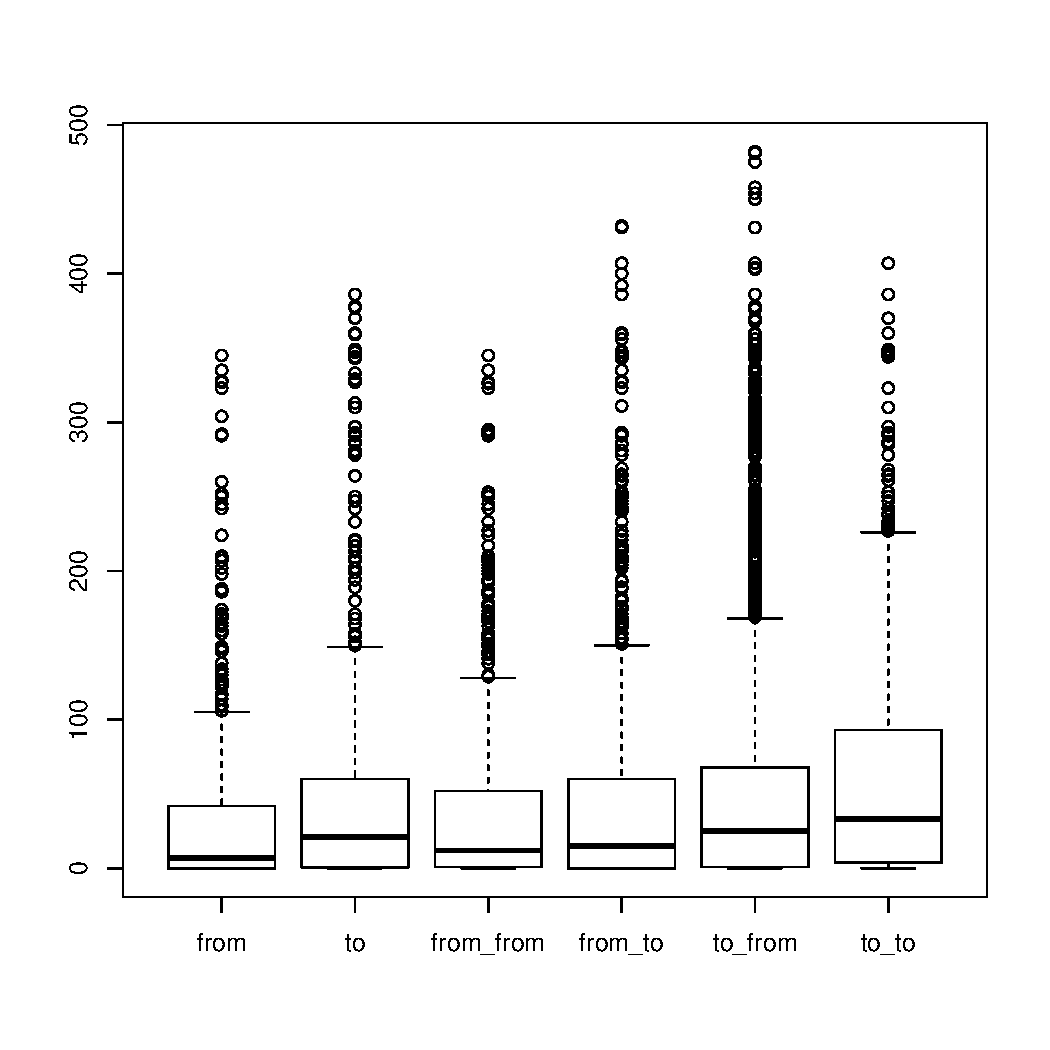
\includegraphics[width=0.95\columnwidth]{date.pdf}
\caption{依存関係の分類ごとの変更時間間隔}
\label{fig:subdate} 
\end{figure}

各依存関係の分類ごとに二標本t検定を行った結果,p値は0.05よりも小さいため,図\ref{fig:subdate}から依存関係別で有意に差があることが判明した.
よって仮定RQ1-1については正しいことが確認できたがRQ1-2は成り立たないことが確認できた.
以下のRQ2,RQ3でも,この依存関係の分類を用いることにする.


%実験・RQ2
\subsubsection*{RQ2:依存関係があるファイル(fがgに依存)の変更において,gが変更されたあとfが変更時間間隔は,fとgの開発者が同じ場合には,異なる場合よりも,短くなる}
依存関係をもつファイルを同じ開発者が変更した場合の変更時間間隔への影響を調査した.
%図\ref{fig:author_true_subdate} は同じ開発者が変更した場合の変更時間間隔を出力している.
%また,図\ref{fig:author_false_subdate} は異なる開発者が変更した場合の変更時間間隔を出力している.
図\ref{fig:author_subdate} は同じ開発者によるコミットと異なる開発者によるコミットの変更時間間隔の箱ひげ図を出力している.


%\begin{comment}
%\begin{figure}
%\centering
%\begin{minipage}{0.49\columnwidth}
%\centering
%\includegraphics[width=\columnwidth]{author_date_TRUE.pdf}
%\caption{同じ開発者の依存関係の分類ごとの変更時間間隔}
%\label{fig:author_true_subdate} 
%\end{minipage}
%\begin{minipage}{0.49\columnwidth}
%\centering
%\includegraphics[width=\columnwidth]{author_date_FALSE.pdf}
%\caption{異なる開発者の依存関係の分類ごとの変更時間間隔}
%\label{fig:author_false_subdate} 
%\end{minipage}
%\end{figure}
\begin{figure}[t]
\centering
\includegraphics[width=0.95\columnwidth]{author.pdf}
\caption{開発者を考慮した依存関係の分類ごとの変更時間間隔}
\label{fig:author_subdate} 
\end{figure}


二つの図を比較した結果,この実験では仮定が正しいことがわかった.

%実験・RQ3
\subsubsection*{RQ3:依存関係があるファイル(fがgに依存)の変更において,gが変更されたあとfが変更時間間隔は,fのコミットが複数のブランチのマージとなったコミットである場合には,そうではないコミットの場合よりも長くなる}
マージとなるコミットの変更時間間隔の影響を調査した.
%図\ref{fig:merge_true_subdate} はマージとなるコミットの変更時間間隔を出力している.
%また,図\ref{fig:merge_false_subdate} はマージではないコミットの変更時間間隔を出力している.
図\ref{fig:merge_subdate} はマージとなるコミットとマージではないコミットの変更時間間隔の箱ひげ図を出力している.
%\begin{figure}
%\centering
%\begin{minipage}{0.49\columnwidth}
%\centering
%\includegraphics[width=\columnwidth]{merge_date_TRUE.pdf}
%\caption{マージとなるコミットの依存関係の分類ごとの変更時間間隔}
%\label{fig:merge_true_subdate} 
%\end{minipage}
%\begin{minipage}{0.49\columnwidth}
%\centering
%\includegraphics[width=\columnwidth]{merge_date_FALSE.pdf}
%\caption{マージではないコミットの依存関係の分類ごとの変更時間間隔}
%\label{fig:merge_false_subdate}
%\end{minipage}
%\end{figure}

\begin{figure}[t]
\centering
\includegraphics[width=0.97\columnwidth]{merge.pdf}
\caption{マージを考慮した依存関係の分類ごとの変更時間間隔}
\label{fig:merge_subdate} 
\end{figure}

二つの図を比較した結果,この実験では仮定が正しいことが分かった.

%考察
\section{考察}\label{考察}

%考察 RQ1
\subsection{RQ1:変更されたファイルに依存関係のあるファイルが変更されるまでの時間は依存関係のないファイルより短くなる}
図\ref{fig:subdate}について考察する.
最も開発期間が長いものがotherであることから依存関係があるものは依存関係の向きや長さを問わず早く変更される傾向にあると考えられる.

\subsubsection*{RQ1-1ファイルfがファイルgに依存するとき,gが変更されたあとfが変更されるまでの時間は,依存関係がないファイルと比較して短い}
dependerやdepender2からわかるように変更されたファイルに依存しているファイルが早く変更される傾向にあることが分かった.
すべてのファイルの変更されるまでの日付の中央値は25日なのに対してdependerは約5日で変更される.
基本的に変更によって影響を受けるものは変更されたファイルに依存関係をもつファイルであることが予測できるため,妥当な結果であるといえる.

\subsubsection*{RQ1-2 ファイルfがファイルgに依存するとき,fが変更されたあとgが変更されるまでの時間は,依存関係がないファイルと同じである}
dependeeやdependee2もotherよりは開発期間が短くなることから, 変更されたファイルに対して依存されているファイルも影響を受けることが分かった.
変更する理由としては変更後に同じ機能を実装した場合や必要なデータが増えたことが予測される.

また,depender2よりもdepender,dependee2よりもdependeeのほうが変更時間間隔が小さくなる.
このことから依存関係の向きだけでなく,依存関係の距離も変更時間間隔に影響を与えていることがわかった.
ただし,dependeeよりもdepender2のほうが変更時間間隔は短い.
以上から,影響の大きい順に依存関係の向き,依存関係の距離が関係していることがわかった.


% 考察 RQ2
\subsection{RQ2:依存関係があるファイル(fがgに依存)の変更において,gが変更されたあとfが変更時間間隔は,fとgの開発者が同じ場合には,異なる場合よりも,短くなる}
図\ref{fig:author_subdate}  について考察する.
同じ人物が変更した場合に中央値が下がることに関して考えられる理由は,同じ開発者が変更したコミットの大部分は同時に変更をしたことがある.
多くの開発者が不具合がでないように他の依存関係のあるファイルを変更するので妥当な結果といえる.
ほかに考えられる理由を以下に示す.
\begin{enumerate}
\item 依存関係をもつ同じパッケージに入っているため変更中に変更の必要性に気づきやすいため同時に変更される
\item 異なる開発者によるコミットの場合前のコミットの理解に時間がかかる
\end{enumerate}
dependee2とotherを比較した場合,異なる人物が変更した場合には大きな差がないのに対して,同じ人物が変更した場合は20日近く差があることが分かった.
原因としてdependee,dependee2のように依存されるファイルは抽象度が高く,異なる開発者による変更は慎重に行われていることが考えられる.

%考察 RQ3
\subsection{RQ3:依存関係があるファイル(fがgに依存)の変更において,gが変更されたあとfが変更時間間隔は,fのコミットが複数のブランチのマージとなったコミットである場合には,そうではないコミットの場合よりも長くなる}
図\ref{fig:merge_subdate} について考察する.

マージとなるコミットの場合マージされていないコミットと比較して次に変更される時期が遅くなる傾向がある.
考えられる理由を以下に示す.
\begin{enumerate}
\item レビューを通してから変更を適用するために信頼性が高く,変更の必要がなくなる
\item マージされ終わり, 作業が減る
\item 変更を行ったのがプロジェクト内の開発者ではないため不具合があったとしても修正に時間がかかる
\end{enumerate}

特にマージされたコミットではdependee2はotherと中央値が近い数値を出している.
考えられる理由を以下に示す.
\begin{enumerate}
\item 外部からの変更ではあまり抽象的になりがちなファイルを変更しづらい
\item 絶対数が少ないため, 変更されにくい
\end{enumerate}

% 妥当性の検証
\section{妥当性の脅威}\label{妥当性の検証}
以下に,本研究における潜在的な妥当性の脅威について議論する.

\subsection*{単一のプロジェクトでの検証}
今回の実験で対象としたプロジェクトはeclipseに関係するオープンソースプロジェクトであるvert.vであった.
比較が容易であると推測されるeclipseに関係するvert.v以外のプロジェクトや,ほかのオープンソースプロジェクトや商業ソフトウェアで,同様結果が得られるとは限らない.
特にソフトウェアの規模によっては開発者の違いや全体的な開発期間に影響があることが予測される.

\subsection*{開発者の専門性についての考慮}
Thongtanunamらは開発者の経験についてレビュー・開発経験についての影響について考慮した研究を行った\cite{Thongtanunam2}.
同じ開発者やマージされた変更であっても開発者の経験によって変更時間間隔に影響が考えられる.

\subsection*{他の依存関係やメトリクスとの比較}
依存関係についての調査では継承や参照もすべて同じ依存関係であるとした.
依存関係の種類\cite{Kotani}別に調査することで変更時間間隔の実験結果が変わる可能性がある.
また,変更波及解析の研究として他に依存関係の構造をもとにしたPropagation Cost(PC)を図る研究などもある\cite{Nord}.
このような過去のメトリクスとの比較をすることで本研究の有効性を理解することができるのではないかと考えている.

\subsection*{dependeeとdependerの関係}
DSM\cite{Nord}ではファイルがお互いに依存しあうことも考慮されている.
そのため本研究では変更されたファイルが依存するファイルであるdependeeと変更されたファイルが依存されるファイルであるdependeeが互いに同じ要素を持っていることが考えられる.
dependeeはdependerにも含まれる要素の影響のみでotherとの差が生まれていることも考えられる.

% まとめ
\section{まとめ} \label{まとめ}
本研究では,オープンソースの分散ソフトウェア開発プロセスのレポジトリを対象として,
ファイルの依存関係が変更時間間隔に与える影響について調査することで,
ファイル間に依存関係による変更の波及があることを実験によって確認した.
さらに,依存関係を遡る向きへの影響や,ファイルを修正した開発者の違い,
コミットがブランチのマージに相当するかどうかの違いが,ファイルの変更時間間隔に与える影響を調査した.
結果,ファイルを修正した開発者が異なること,および,コミットがマージであることが特に変更時間間隔を
長くする要因であることを特定した.
今後は,他のプロジェクトに対しても同様の実験を行い,同じ傾向がみられるかを調査することで,
これが分散ソフトウェア開発プロセスの特徴であるかを確認する必要がある.

\noindent \\
{\bf 謝辞} 本研究はJSPS科研費16K12412の助成を受けたものである.

\begin{thebibliography}{10}
\bibitem{Balachandram}
Balachandran V.,``Reducing Human Effort and Improving Quality in Peer Code Reviews using Automatic Static Analysis and Reviewer Recommendation,'' Proc. the 2013 International Conference on Software Engineering (ICSE '13), pp. 931-940, 2013.

\bibitem{Beszedes}
Besz\'edes, \'A., Gergely, T., Farag\'o, S., Gyim\'othy, T., and Fischer, F.,
``The  dynamic  function  coupling  metric  and  its  use  in  software evolution,'' Proc. the 11th  European  Conference on Software Maintenance and Reengineering (CSMR’07), pp. 103–112, 2007.

\bibitem{Bird}
Bird, Christian, et al. ``Don't Touch My Code!: Examining the Effects of Ownership on Software Quality,'' Proc. the 19th ACM SIGSOFT Symposium and the 13th European Conference on Foundations of Software Engineering (ESEC/FSE '11), pp.4-14, 2011.

\bibitem{Briand}
Briand, L. C., Labiche, Y., O' Sullivan, L., and Sówka, M. M., ``Automated Impact Analysis of UML Models,'' Journal of Systems and Software, Vol. 79, No. 3, 339-352, 2006.

\bibitem{Budgen}
Budgen, D., Burn, A. J., Brereton, O. P., Kitchenham, B. A., and Pretorius, R., ``Empirical Evidence about the UML: a Systematic Literature Review,'' Journal of Software: Practice and Experience, Vol. 41, No. 4, pp. 363-392, 2011.

\bibitem{Canfora}
Canfora, G., Ceccarelli, M., Cerulo, L., and Di Penta, M., ``Using Multivariate Time Series and Association Rules to Detect Logical Change Coupling: An empirical study,'' Proc. the IEEE International Conference on Software Maintenance (ICSM '10), pp. 1-10, 2010.

\bibitem{Kondo}
近藤 和弘, 大畑 文明, 井上克郎, ``オブジェクト指向プログラム変更時の影響波及解析手法の提案,'' 電子情報通信学会技術研究報告. SS-2001-38, Vol. 101, No. 628, pp.33-40, 2002.

\bibitem{Kotani}
小谷 正行, 落水 浩一郎, ``UML 記述の変更波及解析に利用可能な依存関係の自動生成,'' 情報処理学会論文誌, Vol. 49, No. 7, pp.2265-2291, 2008.

\bibitem{Nord}
Nord, R.L., Ozkaya, I., Sangwan, R.S., Delange, J., González, M., Kruchten, P., ``Variations on Using Propagation Cost to Measure Architecture Modifiability Properties,'' Proc. the 29th IEEE International Conference on Software Maintenance (ICSM '13), pp. 400-403, 2013.

\bibitem{Ryder}
Ryder, Barbara G., and Frank Tip, ``Change Impact Analysis for Object-Oriented Programs,'' Proc. the 2001 ACM SIGPLAN-SIGSOFT Workshop on Program Analysis for Software Tools and Engineering (PASTE'01), pp. 46-53, 2001.

\bibitem{Thongtanunam2}
Thongtanunam, P., McIntosh, S., Hassan, A. E. Iida, H., ``Revisiting Code Ownership and Its Relationship with Software Quality in the Scope of Modern Code Review,'' Proc. the 38th International Conference on Software Engineering (ICSE '16), pp. 1039-1050, 2016.

\bibitem{Thongtanunam}
Thongtanunam, P., Tantithamthavorn, C., Kula, R. G., Yoshida, N., Iida, H., Matsumoto, K., ``Who Should Review My Code? A File Location-Based Code-Reviewer Recommendation Approach for Modern Code Review,'' Proc. the 22nd IEEE International Conference on Software Analysis, Evolution, and Reengineering (SANER '15), pp. 141-150, 2015.
%Patanamon Thongtanunam, Chakkrit Tantithamthavorn, Raula Gaikovina Kula, Norihiro Yoshida, Hajimu Iida, Ken-ichi Matsumoto: Who Should Review My Code? A File Location-Based Code-Reviewer Recommendation Approach for Modern Code Review, 22nd IEEE International Conference on Software Analysis, Evolution, and Reengineering, 2015.

% \cite{Patanamon} → \cite{Thongtanunam}
%\bibitem{Patanamon} 
%Patanamon Thongtanunam, etc...
%Who Should Review My Code? A File Location-Based Code-Reviewer Recommendation Approach for Modern Code Review
% \cite{Patanamon2} → \cite{Thongtanunam2}
%\bibitem{Patanamon2}
%Patanamon Thongtanunam1, Shane McIntosh, Ahmed E. Hassan, Hajimu Iida Revisiting Code Ownership and its Relationship with Software Quality in the Scope of Modern Code Review

\end{thebibliography}

\end{document}

